\documentclass[11pt, oneside]{article} 
\usepackage{geometry}
\geometry{letterpaper} 
\usepackage{graphicx}
	
\usepackage{amssymb}
\usepackage{amsmath}
\usepackage{parskip}
\usepackage{color}
\usepackage{hyperref}

\graphicspath{{/Users/telliott_admin/Tex/png/}}
% \begin{center} 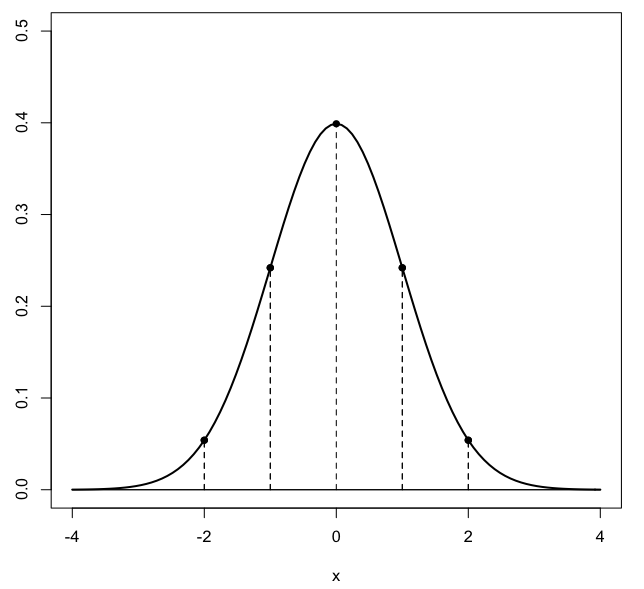
\includegraphics [scale=0.4] {gauss3.png} \end{center}

\title{Average value}
\date{}

\begin{document}
\maketitle
\Large

\label{sec:Average_value}

Consider the problem of the \emph{average value} of a function $f(x)$ over some interval $[a,b]$.  

One way to think of that would be, by analogy to a list of numbers, to collect the values of $f(x)$ at each point along the graph of the function, and then compute the mean.  Of course, there is an infinite number of such points, so that's a bit of a problem.

\begin{center} 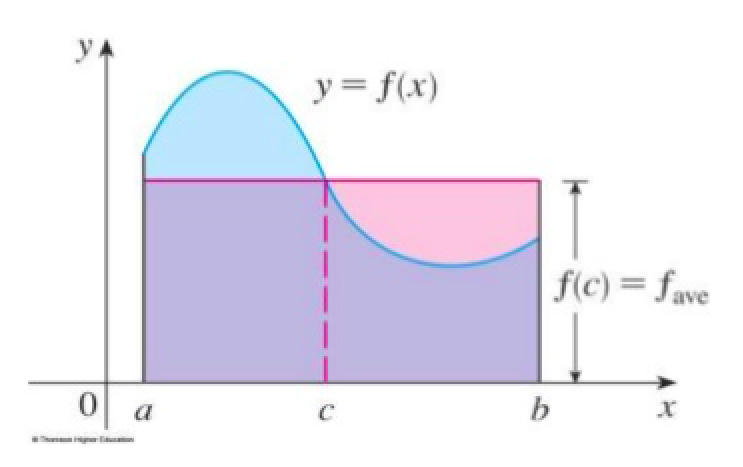
\includegraphics [scale=0.3] {avg_of_func.png} \end{center}

Suppose we integrate, and find the total area under the curve $y = f(x)$ between $x=a \rightarrow x = b$.  Take the number calculated from the definite integral, divide by the distance $b-a$, and plot the result as a height $h$ so as to form a rectangle above the $x$-axis.

Clearly $h$ is a reasonable stand-in for the average value of $f(x)$, since the rectangle formed from $ [a,b] \times [0,h]$ gives the same area as we found under the curve by integration.  Call this $\bar{f}(x)$ ($f$ bar).  Define it to be

\[ \bar{f}(x) = \frac{h}{b-a} \]
\[ =  \frac{\int_a^b f(x) \ dx}{b-a}  \]

The average value of a function over an interval is the integral of the function divided by the length of the interval.  To see the analogy with what we'll do later, write

\[ \bar{f}(x) = \frac{\int_a^b f(x) \ dx}{\int_a^b \ dx}  \]

The denominator is simply the length of the interval.*

\subsection*{example}

\begin{center} 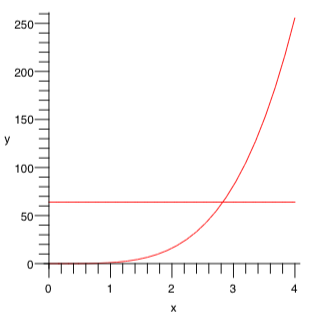
\includegraphics [scale=0.6] {average_value.png} \end{center}

Which is bigger, the rectangle of height $64$ and width $4$ or the area under $x^4$ between $0$ and $4$?

We integrate $\int x^4$ and obtain $x^5 / 5$ evaluated between $0$ and $4$, giving $4^5/5$ or $4^4 \times 0.8$.  This is just smaller than the area of the rectangle which is $4^3 \times 4$.  

The average value of the function $f(x) = x^4$ over this interval is $0.8 \times 4^3$, obtained by dividing the result of the integral by the length of the interval.

\subsection*{mean value theorem}

It is worth pointing out that the \textbf{mean value theorem for integrals} states if $h = \int f(x) \ dx$ over the interval $[a,b]$, there is at least one value $x_0$ in the same interval, such that $f(x_0) = h$.

\subsection*{geometric centroid of a triangle}

Next, we want to know, what is the position of the average point inside some geometric figure.  That point is called the centroid.  For example, where is the average point in a triangle?  For a physical object with constant density, the centroid would be the \textbf{center of mass}.

If we consider a right triangle having its base along the $x$-axis, and we call that length $B$, then the height would be $H$.  Let the pointy end be at the origin, and the equation of the line describing the bounding line of the triangle is $y = H/B \cdot x$.

One reason to do the triangle as an example is that we already know the answer.  Ceva's theorem tells us that the centroid is $2/3$ of the way toward the fat end, for both $x$ and $y$.

\begin{center} 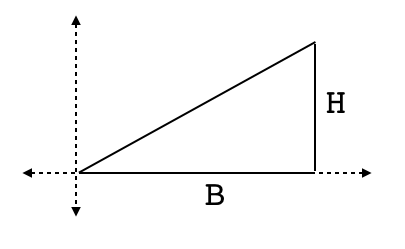
\includegraphics [scale=0.5] {simple_triangle.png} \end{center}

In trying this problem, I first thought, what is the average value of $y$? Maybe it's 
\[ \bar{y} \stackrel{?}{=} \int_0^B y \ dx \]

This turns out not to be correct.  It gives what we asked for, the average value of $y$, the distance of the upper edge from the $x$ axis, times $x$.  The result is the area of the triangle.

\[ = \int_0^B \frac{H}{B} x \ dx \]
\[ = \frac{H}{B} \ \frac{x^2}{2} \ \bigg |_0^B \]

That's not what we're looking for.

Surely $\int x \ dx$ is not right either.  It will turn out that $\int xy \ dx$ is the answer.  This approach is suggested by extending the idea of average value from above into two dimensions.  We had

\[ \bar{f}(x) = \frac{\int_a^b f(x) \ dx}{\int_a^b \ dx}  \]

Substitute

\[ \bar{f}(x,y) = \frac{1}{A} \ \iint f(x) \ dA \]
\[ = \frac{\iint f(x) \ dA}{\iint \ dA} \]

where $A = \iint dA$ is the total area.

To get the average of value of the $x$-coordinate, just do (leaving the area $A$ aside for the moment):

\[ \iint f(x) \ dA = \int \int x \ dy \ dx \]

We decide we will do $\int dy$ first and go back to the figure to get $y$ as a function of $x$:

\[  \int_{x=0}^{x=B} \int_{y=0}^{y=Hx/B} x \ dy \ dx \]

The inner integral is simply
\[ \int_{0}^{Hx/B} x \ dy = xy \ \bigg |_{0}^{Hx/B}  \]
\[ = Hx^2/B \]
and the outer integral is
\[ \int_{0}^{B} \frac{H}{B} x^2 \ dx =  \frac{H}{B} \ \frac{x^3}{3}  \ \bigg |_{0}^{B}  \]
\[ = \frac{HB^2}{3}  \]

The last step is to divide by the area $A = HB/2$, obtaining 

\[ \frac{HB^2}{3} \ \frac{2}{HB} = \frac{2}{3} \ B  \]

which is correct.

The question is, can we see anything that would be useful for expressing this idea in terms of one-variable calculus?

The inner integral is $\int x \ dy$ with \emph{constant} $x$, or just $xy$.

We weight the value of $x$ at every point along the base by the number of points with each $x$, namely, $y$.  The integral is
\[ \int xy \ dx \]
and we will need to correct at the end by
\[ \int y \ dx \]
which is the area.  To restate this:
\[ \bar{x} = \frac{ \int xy \ dx}{\int y \ dx} \]

The average point in this right triangle lies $2/3$ of the base away from the pointy end.  By symmetry, the same is true for $y$.  This is \hyperref[sec:Ceva]{\textbf{Ceva's Theorem}}.

\subsection*{geometric centroid of a half-circle}

Consider a half-circle of radius $R$ centered at the origin (just the part above the $x$-axis).  We compute the average values of $x$ and $y$

\[ \bar{x} = \frac{1}{A} \ \iint x \ dA \]
\[ \bar{y} = \frac{1}{A} \ \iint y \ dA \]

By symmetry, it's clear that $\bar{x} = 0$.  Let's compute it anyway.  Since we do have the $x$, we should keep Cartesian coordinates.  We integrate with respect to $y$ first:
\[ \int_{-R}^{R} \int_0^{\sqrt{R^2-x^2}} x \ dy \ dx \]

The inner integral is
\[ xy \ \bigg |_0^{\sqrt{R^2-x^2}} \]
\[ = x \sqrt{R^2-x^2} \]

The outer integral is
\[ \int_{-R}^{R} x \sqrt{R^2-x^2} \ dx \]
\[ = - \frac{1}{3} \ (R^2-x^2)^{3/2} \ \bigg |_{-R}^R = 0 \]
This is an even function of $x$ so any integral centered about $0$ has the same value at both bounds and the value is just zero.  

The area is $\pi$ but zero times $1/\pi$ is still zero.  

The average value of $y$ over the circle is calculated as follows.
\[ \int_{-R}^{R} \int_0^{\sqrt{R^2-x^2}} y \ dy \ dx \]

We can do this in Cartesian or polar coordinates.  For the first way the inner integralis
\[  \int_0^{\sqrt{R^2-x^2}} y \ dy = \frac{y^2}{2} \ \bigg |_0^{\sqrt{R^2-x^2}} \]
\[ = \frac{R^2 - x^2}{2} \]
The outer integral is
\[ \int_{-R}^{R} \frac{R^2 - x^2}{2} \ dx \]
\[ = \frac{1}{2} \ [ \ R^2x - \frac{x^3}{3} \ ] \ \bigg |_{-R}^{R} \]
\[ = \frac{1}{2} \ [ \ (R^3 - \frac{R^3}{3}) - (-R^3 - -\frac{R^3}{3}) \ ] \]
It's hard to keep track of the minus signs.  
\[ = \frac{1}{2} \ [ \ (2R^3 - 2\frac{R^3}{3} \ ] \]
\[ = \frac{2}{3} R^3 \]

If you dare, realize that this
\[ \int_{-R}^{R} \frac{R^2 - x^2}{2} \ dx \]
is an even function of $x$, so we can change the lower bound to zero and multiply by $2$:
\[ = 2 \int_{0}^{R} \frac{R^2 - x^2}{2} \ dx \]
The $2$ conveniently cancels and we have
\[ \ R^2x - \frac{x^3}{3} \ \bigg |_{0}^{R} \]
which gives the correct answer painlessly.

Perhaps we do want to switch to polar coordinates.  I am tempted to write:
\[ y = R \sin \theta \]

but that is not correct!  I need a variable $r$
\[ y = r \sin \theta \]

So $dA$ becomes:
\[ dA = dy \ dx = r \ dr \ d \theta \]
and we have
\[ \iint y \ dA = \int_0^{\pi} \int_0^R r \sin \theta \ r \ dr \ d \theta \]
\[ = \int_0^{\pi} \int_0^R \sin \theta \ r^2 \ dr \ d \theta \]

The inner integral is
\[ \int_0^R \sin \theta \ r^2 \ dr = \sin \theta \int_0^R  r^2 \ dr \]
\[ = \sin \theta \ \frac{R^3}{3} \]

So the outer integral is
\[ \frac{R^3}{3} \int_0^{\pi} \sin \theta  \ d \theta \]
\[ \frac{R^3}{3} \ [ \ - \cos \theta \ \bigg |_0^{\pi} \ ] = \frac{2R^3}{3} \]

However, this integral for the numerator is obtained, remember to divide by $(1/2)\pi R^2$ to obtain
\[ \frac{2R^3}{3} \cdot \frac{2}{\pi R^2} = \frac{4R}{3 \pi} \]

The geometric centroid of a half-circle is at $(0, 4R/3 \pi$).  This is not so obvious.  It will become very useful when we consider Pappus Theorem later on.

\subsection*{problem}
There is a problem in Varberg that has an easy solution and a hard solution.  We've done part of the easy solution here, and the reason I know this is Auroux shows the answer.  Varberg does only the hard calculation, which is a little weird.

\begin{center} 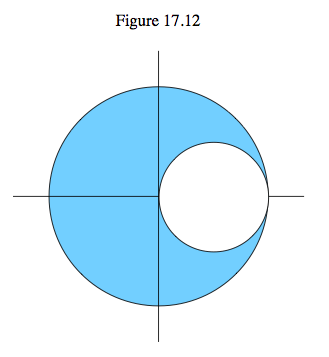
\includegraphics [scale=0.6] {Varberg17-12.png} \end{center}

The diagram shows the unit circle at the origin in blue with an inset circle in white that has been removed.  The missing circle has radius $1/2$ and is centered at $1/2,0$.  The problem is to find the average value of the function $x$ over the blue region.

Now, we've just finished showing that the average value of $x$ over the unit circle is zero.  But $\bar{x}$ over the small circle will not be zero, and we will obtain minus that value by subtracting from the big circle.  

\[ \bar{x} = \frac{1}{Area} \ \iint_R x \ dA \]

Since surely $\bar{x}$ over the small circle is at the origin, $x = 1/2$, multiplied by the area $\pi/4$ and negated because of the subtraction, we predict the answer will be $- \pi/8$.

Let's try to do the problem the way it's done in Varberg.

The idea is to use polar coordinates.  It's really hard to see how you could possibly do it in Cartesian coordinates, except in the way that we already used them.  How do we describe the $x$-dependence of the bounds on $y$?  I suppose we could try, but let's go with polar.  

We will integrate the top half of the circle, and we'll do it separately for the first and second quadrants.

\[ \int \int x \ r \ dr \ d \theta \]
\[ x = r \cos \theta \]
\[ \int \int r \cos \theta \ r \ dr \ d \theta \]

Pretty standard.  We will integrate with respect to $\theta$ last.  So, now our job is to figure out how what the lower limit is on $r$ as $\theta$ varies.

\begin{center} 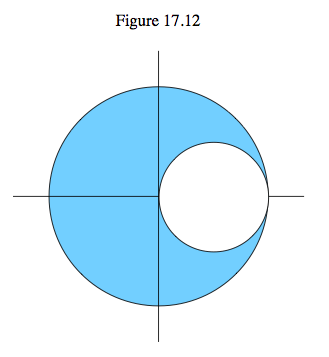
\includegraphics [scale=0.6] {Varberg17-12.png} \end{center}

For the lower limit, when $\theta = 0$, $r = 1$.  And when $\theta = \pi/2$, $r = 0$. I don't know how you could be sure it works everywhere if you didn't know the answer, but $\cos \theta$ is correct.
 
We'll come back to the issue of how this was found later.  Let's calculate:

\[ \int_0^{\pi/2} \int_{\cos \theta}^{1} r \cos \theta \ r \ dr \ d \theta \]

The inner integral is

\[ \frac{r^3}{3} \cos \theta \ \bigg |_{\cos \theta}^{1} \]

So the outer integral is then

\[ \frac{1}{3} \int_0^{\pi/2} \cos \theta - \cos^4 \theta  \ d \theta \]

So we will have an outside factor of $1/3$ and $\sin \theta$ between $0$ and $\pi/2$, which is just 1, but we have to deal with the fourth power of the cosine.  Not fun. We make repeated application of the double-angle formula:

\[ \cos^2 s = \frac{1}{2} (1 + \cos 2s) \]
\[ \cos^4 s = \frac{1}{4} (1 + \cos 2s)^2 \]
\[ = \frac{1}{4} (1 + 2 \cos 2s + \cos^2 2s) \]

Substitute $t = 2s$
\[ \cos^2 2s = \cos^2 t = \frac{1}{2} (1 + \cos 2t) \]
\[ = \frac{1}{2} (1 + \cos 4s) \]
Substitute back to the previous version

\[ \frac{1}{4} (1 + 2 \cos 2s + \cos^2 2s) \]
\[ = \frac{1}{4} (1 + 2 \cos 2s + \frac{1}{2} (1 + \cos 4s)) \]

Rearrange slightly

\[ = \frac{3}{8} + \frac{1}{2} \cos 2s + \frac{1}{8} \cos 4s \]

Substitute $\theta$, integrate and get 

\[ = \frac{3}{8}\theta + \sin 2 \theta + \frac{1}{2} \sin 4 \theta \]

With limits of $\theta = 0 \rightarrow \pi/2$ we have only the first term and that one only at the upper limit

\[  = \frac{3}{16} \pi \]

Combine it with the rest of the integral to obtain

\[ \frac{1}{3}(1 - \frac{3}{16} \pi ) \]

Now, on to the second quadrant.

\[ \int_{\pi/2}^{\pi} \int_{0}^{1} r \cos \theta \ r \ dr \ d \theta \]

The inner integral is 

\[ \frac{1}{3} r^3 \cos \theta \ \bigg |_0^1  \]
\[ = \frac{1}{3} \cos \theta \]

And the outer integral is then

\[   \frac{1}{3}  \int_{\pi/2}^{\pi} \cos \theta \ d \theta \]

which is just $-1/3$.  So finally, we add them up:

\[ \frac{1}{3}(1 - \frac{3}{16} \pi ) - \frac{1}{3} = - \frac{\pi}{16} \]

Recall that we integrated only the top half of the figure, so multiply by $2$ to obtain the same answer that we had much more simply before!

\subsection*{insight}

The part I like about this problem is seeing the limits on $r$.  The equation of a circle in polar coordinates is given as

\[ r = a \cos \theta + b \sin \theta \]

where $(a/2,b/2)$ is the center of the circle.  Since $b = 0$ (we're on the $x$-axis with $y = 0$), and $a = 1$, the small circle has the equation

\[ r = \cos \theta \]

How to check that?  Well, we can convert from polar to Cartesian like this.  Multiply the equation for the circle by $r$:
\[ r^2 = r \cos \theta \]
Since $x = r \cos \theta$
\[ r^2 = x \]
But $r^2$ is also equal to $x^2 + y^2$ so
\[ x = x^2 + y^2 \]
\[ x^2 - x + y^2 = 0 \]
 
Complete the square:

\[ x^2 - x + \frac{1}{4} + y^2 = \frac{1}{4} \]
\[ (x - \frac{1}{2})^2 + y^2 = \frac{1}{4} \]

This is indeed our circle, a circle of radius $1/2$ centered at $O = (1/2,0)$.

Going back to the polar equation of the small circle $r = \cos \theta$, we can think of this as having $\theta$ in sync for the two circles.

As we advance the parameter $\theta$ for the large circle, we can find the position of $r$ (where the point is with respect to the origin), at the same value of $\theta$ for the small circle.  At least, that's how it seems to me.

We have to remember that for an off-center circle (not at the origin) in polar coordinates the $r$ parameter is still with respect to the origin, rather than with respect to the center of the circle.

\end{document}  